\documentclass{beamer}
\usepackage{lsfolien}
\usepackage[english]{babel}
\usepackage[utf8]{inputenc}

\myfootline{System Modelling and Semantic Web -- Spring 2021}{Hans-Gert Gräbe}

\newcommand{\ueberschrift}[1]{\begin{center}\bf #1\end{center}}

\title{Modelling Sustainable Systems\\ and Semantic Web\\[6pt] Knowledge and
  Action \vskip1em}

\subtitle{Lecture in the Module 10-202-2309\\ for Master Computer Science}

\author{Prof. Dr. Hans-Gert Gräbe\\
\url{http://www.informatik.uni-leipzig.de/~graebe}}

\date{July 2021}
\begin{document}

{\setbeamertemplate{footline}{}
\begin{frame}
  \titlepage
\end{frame}}

\section{Storytelling and Digital Change}
\begin{frame}{Storytelling and Digital Change. Summary}

Starting point: RDF -- what is happening there and in general in the internet?
\begin{itemize}
\item It is a digital form of storytelling.
\item Storytelling accompanies our \emph{cooperative actions}. Cooperative
  actions are possible only in such an interpersonal language based context.
\item Question (1): \emph{What} is here conveyed by language?
\item But: Storytelling is not reduced to its \emph{communicative} function.
  It has also a \emph{reflective} component.
\item Question (2): How does \emph{theory building} work on such an empirical
  background?
\item There is an arc of tension \emph{Justified expectations $\to$ World
  changing actions $\to$ Experienced results}
  \begin{itemize}
  \item Interpersonally this arc of tension is to be explored only
    in language form and \emph{only in specific contexts}.
  \end{itemize}
\end{itemize}
\end{frame}

\begin{frame}{Storytelling and Digital Change. Summary}
Why act cooperatively? "Change the world".
\begin{itemize}
\item But how change a world that is also constantly changing itself?  How to
  deal with the diversity and contradictions of the requests for change?
\item Approach "influence the changes of the world".
  \begin{itemize}
  \item "Doing" is embedded here, prior to it is the reality of life.
    Justified expectations can only be derived from this reality of life.
\item Experience: \emph{Practical} influence is (today) only possible through
  application of adequate processual knowledge and processual skills.
  \end{itemize}
\item But why cooperate?
  \begin{itemize}
  \item Cooperative action is more powerful than individual action due to
    emergent synergistic effects.
  \item The whole is more than the sum of its parts.
  \end{itemize}
\end{itemize}
\end{frame}

\begin{frame}{Storytelling and Digital Change. Summary}
Cooperative action is only possible in a \emph{common context of meaning}.
\begin{itemize}
\item Experience: \emph{Understanding} language presupposes a common context
  of meaning on the one hand, and continues it on the other.
\item This context of meaning expresses itself above all in the \emph{social
  use of common terminology in common activities}.
\item Question (3): How can that itself be expressed in language form?
\end{itemize}
\end{frame}
\begin{frame}{Storytelling and Digital Change. Summary}
Experience: Such contexts of meaning are stabilised through
\emph{institutionalisation}. Meanings are tied to social practices as a
specific interaction between logos and telos.
\begin{itemize}
\item The \emph{practically approved} is socially secured and
  institutionalised as \emph{processual knowledge} (technology) and
  \emph{approved practices}.
\item Question (4): How to set up the notion of \emph{knowledge} in this
  context?
\end{itemize}\vspace*{2em}
\end{frame}
\begin{frame}{Storytelling and Digital Change. Summary}
Observation: Such institutionalized contexts of meaning are nested and
interlaced in many ways.
\begin{itemize}
\item Experience: Cooperation between cooperative structures requires
  translation between contexts of meaning.

  This is yet hardly understood in the field of semantic technologies.
\item People are involved in cooperative contexts with partial identities only
  $\to$ concept of roles.
\end{itemize}
The core of all four questions: How does such an institutionalisation of
contexts of meaning work?
\end{frame}

\begin{frame}{Storytelling and Digital Change. Summary}
\begin{itemize}
\item We also identified this question as a core problem of semantic
  technologies.
\item Historically in the last 150 years there have been various attempts to
  this problem.
\end{itemize}

Attempts to develop a general language theory as Universal Theory.
\begin{itemize}
\item Logical positivism of the Vienna Circle (1920s).
\item Syntax, semantics, pragmatics (Charles W. Morris, 1940)
\item Continuation as semiotics and linguistics in the 1970s.
\item Noam Chomsky and his approach to a universal grammar.
\end{itemize}
\end{frame}

\begin{frame}{Storytelling and Digital Change. Summary}
At the same time, since 1920, increasing importance of evolutionary
approaches: Institutionalisations of contexts of meaning are hierarchically
complex and can be unterstood only in their historical-cultural development.
\begin{itemize}
\item Biosemantics: focus on coevolution of neural patterns and evolutionary
  patterns of contexts of meaning.
\end{itemize}
Pragmatics: Terms develop with their interactive use.  (Jacob L. Mey:
Pragmatics, 1993)
\begin{itemize}
\item The development of concepts cannot be detached from their practical use,
  in particular forms and practices of judgment and judgment.
\end{itemize}
\end{frame}

\section{What is Knowledge?}
\begin{frame}{What is Knowledge?}
  
Stabilization of contexts of meaning through institutionalisation: what has
been \emph{practically approved} is transferred to \emph{processual knowledge}
(technology) and thus socially fixed in \emph{approved practices}.

How is the term knowledge to be understood in this context?

What is knowledge?

\begin{itemize}
\item A cumulative notion as in a knowledge pyramid approach (Aamodt, Nygard
  1995) was already criticised.
\item The debate is heavily influenced by the accumulation theory of knowledge
  developed within linguistics in the 1970s.
\item An inderstanding of knowledge as tangible resource was prominently
  present once more in the discussions about an approriate concept of
  information around 2000.
\end{itemize}
\end{frame}

\begin{frame}{Storytelling, Conceptual Systems, Knowledge}

Storytelling is tied to \emph{interpersonal contexts of meaning}.

\textbf{What is meaning?}
\begin{itemize}
\item Meaning \emph{is} the use of terms.
\item Terms are a form of \emph{cooperative human practices} and thus to be
  contextualized in a concrete-historical manner.
\item Context of a civil society as legal system in which the actors are made
  individually responsible for the consequences of their actions.
\item Action is thus embedded in the updating of interpersonal \emph{relations
  of reasoning} (Begründungszusammenhänge) and \emph{judgment practices}
  (Urteilspraxen).
\end{itemize}
\end{frame}
\begin{frame}{Knowledge According to Berger/Luckmann}

We have rejected a concept of knowledge, which considers knowledge as external
and preceding human action epistemic entity (approach "knowledge pyramid",
cumulative concept of knowledge of linguistics and semiotics).

Another approach is rooted in the sociology of knowledge.  (Berger/Luckmann
1966) develop a concept of knowledge starting from its social use.
\begin{itemize}
\item Knowledge as socially objectified and therefore legitimate
  \emph{interpretation of sense}.
\item Also to be viewed critically. How far reaches a sociological approach of
  knowledge as objectification and mounting of subjectively pre-formed
  interpretations?
\item How stabilisation and institutionalisation of contexts of meaning are
  developed in such a concept?
\end{itemize}
\end{frame}

\begin{frame}{Forms of Knowledge Practices}
  
What has been practically approved becomes processual knowledge and is
institutionalised as approved practices.

Which types of practices are relevant at all?
\begin{itemize}
\item Wide range of forms: general knowledge -- special knowledge -- calculus
  -- skills -- technology.
\item Experience: massive devaluation of knowledge (of entire professions)
  during technological progress argues against a cumulative picture of
  knowledge.
\item "Big data" and "digitization of the world" produces the opposite picture
  -- quantity instead of quality is required?
  \begin{itemize}
  \item But: Successful semantic projects work on a digital reconstruction of
    contexts of meaning in order to make them accessible for the use of
    digital tools.
  \end{itemize}
\end{itemize}
\end{frame}
\begin{frame}{Forms of Institutionalization of Knowledge}
  
Phenomenon of mounting proven structures through "pattern formation"
(Musterbildung), "institutionalisation", "meaning formation"
(Bedeutungsbildung).

But that is only a complexity-reducing one form of description (a
\emph{production of fiction}), because\vspace{-1em}
\begin{itemize}
\item The investigation of the dynamics of the \emph{relations} on the macro
  level assumes a relatively constant structure at the micro level.
  \begin{itemize}
  \item This is valid at least in "normal times" (cf. T. Kuhn's notion of 
    "normal science").
  \end{itemize}
\item "Enslavement effect": macro structures (as context) have a stabilizing
  impact on the dynamics and thus the stability of structures at the micro
  level.  Throughput defines the inner structure of a system.  
\item Approach of a co-evolution model.
\end{itemize}
\end{frame}

\section{Cooperative Action}
\begin{frame}{Knowledge and Cooperative Action}\small
  
The considerations concentrate on a systemic model, i.e. the interweaving of
the dynamics as well as structure and pattern formation processes on the micro
and macro levels and thus on the dynamics of the \emph{internal relations} of
a cooperative context, which is separated from the \emph{outside world} by a
\emph{system boundary}.

Such an approach is a \emph{methodical approach to complexity reduction} by
dividing all possible relationships into three groups,\vspace{-1em}
\begin{itemize}
\item the relations within the system boundaries -- internal relations,
\item the cross-border relations and
\item the relations outside the system -- external relations.
\end{itemize}\vspace{-1em}
The relations in the groups differ in the mode of shapeability related to a
concrete cooperative action.

\textbf{Focus of consideration:} Contexts of meaning unfold in the field of
tension between \emph{justified expectations} and \emph{experienced results}
which develops itself in time.\vskip2em
\end{frame}

\begin{frame}{Yesterday -- Today -- Tomorrow}
\begin{itemize}
\item The (processed) \emph{experienced results} are anchored in the World
  View and thus are a conditionality of further action.  They are a reflex of
  the Yesterday in the Today.
\item The \emph{justified expectations} are based in the World View as a
  reflex of the Tomorrow in the Today.
\item Yesterday: justifications, action planning, development of
  \emph{competence to act}.
\item Today: execution of action 
  \begin{itemize}
  \item It is time critical! Acting under "incomplete information".
  \item \emph{Private} decision-making, action, responsibility.
  \item To enable this condition of possibility are to be \emph{socially}
    produced: Manageability, trust, reliability
  \end{itemize}
\item Tomorrow: The justified expectations are compared with the experienced
  results.
\end{itemize}
\end{frame}

\begin{frame}{Yesterday -- Today -- Tomorrow}
Reasonable expectations\vspace{-1em}
\begin{itemize}
\item The diversity of private expectations appears socially as
  multi-optionality of expected future development.
\end{itemize}\vspace{-1em}
Lessons learned: comparison of the results of action with the expectations.
Further development of \emph{experienced results}.
\begin{itemize}\vspace{-1em}
\item Common experiences are the basis of the further development of the
  \emph{cooperative world view}.
\end{itemize}\vspace{-1em}
Two central mediation contexts for \emph{synchronicity} of cooperative action:
\begin{itemize}\vspace{-1em}
\item Mediation on the level of reasoning as further social development of a
  common World View (and thus of \emph{competence} to act).
\item Mediation on the level of action as socially based further development
  of \emph{shaping reality}.
\end{itemize}
\end{frame}

\begin{frame}{Yesterday -- Today -- Tomorrow}

  \begin{center}
    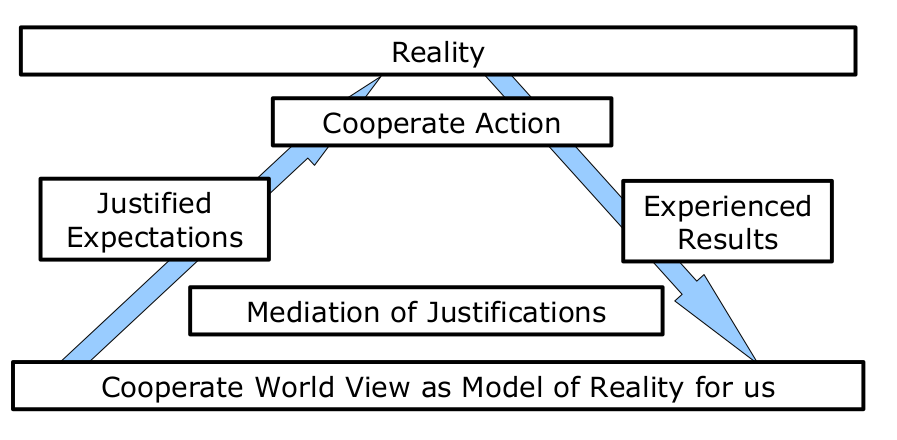
\includegraphics[width=.9\textwidth]{KA-1.png}
  \end{center}
  
This picture describes the position of the two mediation contexts of the
dynamics of cooperative action both at the micro level and the macro level.
\end{frame}

\begin{frame}{Cooperative Action}

  \begin{minipage}{.5\textwidth}\small
  How do justified expectations develop in the context of cooperative action?
  
\textbf{Forms?} Common interests, pre-defined norms.

\textbf{Dynamic moments?} Generalise and spread the approved as commonly
accepted processual knowledge, marginalize or criticize the non approved.

\textbf{Structural Moments?}  \emph{Operationalisation} of processural
knowledge in institutions, tools or technology.  Corporate identity.
  \end{minipage}
\hfill
  \begin{minipage}{.47\textwidth}
  \begin{center}
    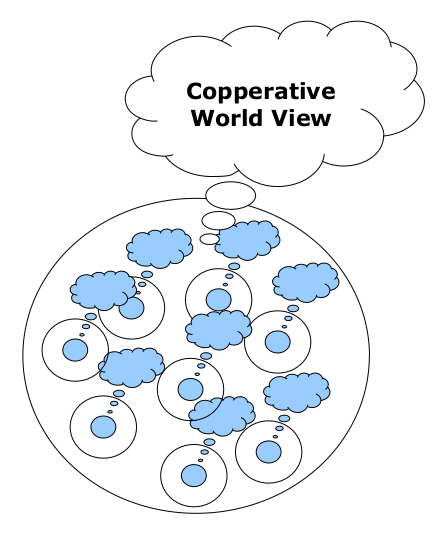
\includegraphics[width=\textwidth]{KA-2.png}
  \end{center}
  
  \end{minipage}
\end{frame}

\begin{frame}{Cooperative Action. Observations}
Relational moments as relationships between actors shape the cooperative
context more than individual moments of individual actors.\vspace{-1em}
\begin{itemize}
\item This requires to postulate also \emph{specific, cooperative processual
  knowledge} that cannot be assigned to individual actors. Such phenomena
  cannot be described within an accumulative concept of knowledge.
\end{itemize}
Actors are involved in cooperative contexts only with partial identities. Or,
interpreted submersively: only in a reduced form of their overall personality.
\vspace{-1em}
\begin{itemize}
\item Such a \emph{reductionistic approach} to the individual personality
  hides intercooperative phenomena of the intentionality of personalities and
  leads to the assumption of a \emph{relational intentionality}.
\end{itemize}
\end{frame}

\begin{frame}{Micro Level: Private Actions of the Actors}
The great importance of private action results from the legal basic
constellation and various institutionalisations of the civil society in which
the consequences of actions can be attributed.

In the field of tension of private action between expectations and results
evolve\vspace{-1em}
\begin{itemize}
\item The private \emph{capability} to act (Handlungsfähigkeit) as
  socio-technical \emph{capacity} to act (Handlungsvermögen) in a socially
  determined \emph{field of action} (Handlungsfeld).
\item The \emph{private World View} (as "Unity of Consciousness") as a reflex
  on the \emph{conditionalities} of this capability to act.
\end{itemize}\vspace{-1em}
In a theory of the \emph{inner perspective of cooperative action} (within the
systemic limit) these processes are visible only so far as they \emph{relate
  to the cooperative context} (reductionistic assumption of relational
intentionality).
\end{frame}

\end{document}
